\section{Introducci\'on te\'orica}

Dado que la modelización utlizada para este problema es una matriz y que en base a algunos datos que nos dan de ella (posición de las saniguijuelas, dimensiones y temperatras de los bordes) tenemos que calcular los valores de muchas celdas, lo que hay que resolver es un sistema de ecuaciones. 
Lo primero que se nos viene a la mente cuando tenemos esto es el método de eliminación gaussiano. Este transforma la matriz de coeficientes en una matriz triangular superior y luego mediante back substitution se pueden obtener todos sus valores.

Veamos ahora más en detalle como funciona cada uno de estos algoritmos.

\subsection{Algoritmo de eliminación gaussiana}
Es importante en este punto aclarar que para poder hacer estos cálculos la martiz debe ser cuadrada (\ref{sec:MatrizCuadrada}).
Los pasos a seguir en este algoritmo son:

\begin{itemize}

\item Ir a la columna no cero extrema izquierda
\item Si el primer renglón tiene un cero en esta columna, intercambiarlo con otro que no lo tenga
\item Luego, obtener ceros debajo de este elemento delantero, sumando múltiplos adecuados del renglón superior a los renglones debajo de él
\item Cubrir el renglón superior y repetir el proceso anterior con la submatriz restante. Repetir con el resto de los renglones (en este punto la matriz se encuentra en la forma de escalón)
\item Comenzando con el último renglón no cero, avanzar hacia arriba: para cada renglón obtener un 1 delantero e introducir ceros arriba de éste sumando múltiplos 
correspondientes a los renglones correspondientes

\end{itemize}
 
Ejemplo:

\begin{figure}[htb]
\begin{center}
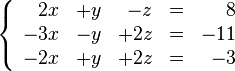
\includegraphics[scale=0.70]{imagenes/ejemplo_gaus_1.png} 
\caption{Sistema de ecuaciones de 3x3} 
\end{center}
\end{figure}

\begin{figure}[htb]
\begin{center}
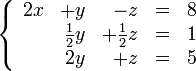
\includegraphics[scale=0.70]{imagenes/ejemplo_gaus_2.png} 
\caption{Sistema de ecuaciones con ceros en la primera columna} 
\end{center}
\end{figure}

\begin{figure}[htb]
\begin{center}
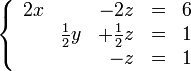
\includegraphics[scale=0.70]{imagenes/ejemplo_gaus_3.png} 
\caption{Sistema de ecuaciones triangulado} 
\end{center}
\end{figure}
\newpage
En esta última imagen podemos observar que el valor de Z ya lo tenemos. Por lo tanto si reemplazamos el mismo en la ecuación arriba obtenemos Y y lo mismo con la primer ecuación.

La complejidad computacional de esto es aproximadamente $n^3$. Esto es, el número de operaciones requeridas es $n^3$ si el tamaño de la matriz es n x n. Por lo tanto puede volverse un cálclo sumamente grande si la matriz es de dimensiones importantes. Por esto decidimos pensar un poco mejor la situación y encontrarle la vuelta para resolverlo en un tiempo razonable. 

\subsection{Matriz banda}

Analizando la matriz del sistema de ecuaciones que se genera a partir de la representación del Parabrisas observamos que presenta las caracteristicas de un tipo de matriz llamada "banda", la cual se distingue por tener todas las celdas en 0 salvo en la diagonal ensanchada, es decir, que p celdas a la izquierda y q a la derecha de la diagonal a lo sumo tienen algunos o todos los valores distintos de 0. En nuestro caso, al construir la matriz nos basamos en el tipo de celda, si es el borde frío o una sanguijuela el coeficiente respectivo sera un 1 en la diagonal igualado a la temperatura correspondiente, pero en el caso de ser una celda vacía en la diagonal irá un -4, a los costados un 1 y representando la fila de "arriba" y "abajo" del parabrisas iran un 1 a "m" columnas de distancia de la diagonal. Finalmente la matriz resultante quedará con una banda de ancho m+m, con "m" el ancho del parabrisas.

Aca podemos ver un ejemplo de una matriz banda:

\begin{figure}[htb]
\begin{center}
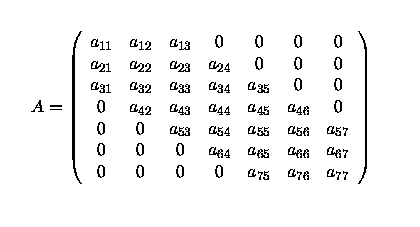
\includegraphics[scale=0.70]{imagenes/matriz_banda.jpg} 
\caption{Matriz banda 7x7} 
\end{center}
\end{figure}







